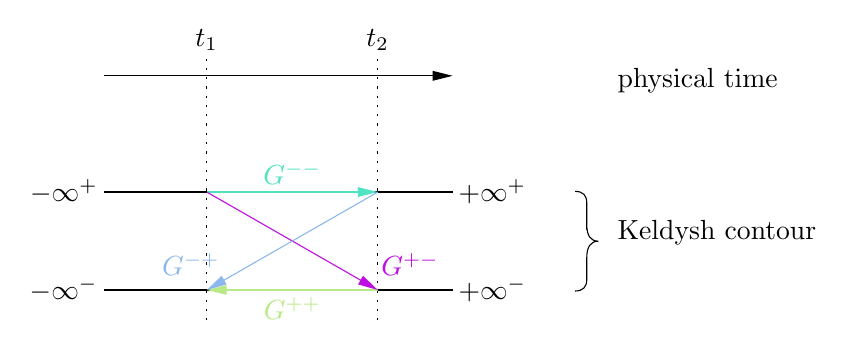
\begin{tikzpicture}[x=0.75pt,y=0.75pt,yscale=-0.8,xscale=0.8]
    %uncomment if require: \path (0,300); %set diagram left start at 0, and has height of 300
    
    %Straight Lines [id:da9923247639127166] 
    \draw    (144,152) -- (354.17,152) ;
    %Straight Lines [id:da5829772718809481] 
    \draw    (144,211) -- (354.17,211) ;
    %Straight Lines [id:da04548734740797422] 
    \draw  [dash pattern={on 0.84pt off 2.51pt}]  (206,71.6) -- (206,229) ;
    %Straight Lines [id:da1610984974972618] 
    \draw  [dash pattern={on 0.84pt off 2.51pt}]  (309,71.6) -- (309,229) ;
    %Straight Lines [id:da04350669910867855] 
    \draw    (144,82) -- (352.17,82) ;
    \draw [shift={(354.17,82)}, rotate = 180] [fill={rgb, 255:red, 0; green, 0; blue, 0 }  ][line width=0.08]  [draw opacity=0] (12,-3) -- (0,0) -- (12,3) -- cycle    ;
    %Shape: Brace [id:dp6257369686518601] 
    \draw   (428,211.6) .. controls (432.67,211.6) and (435,209.27) .. (435,204.6) -- (435,191.6) .. controls (435,184.93) and (437.33,181.6) .. (442,181.6) .. controls (437.33,181.6) and (435,178.27) .. (435,171.6)(435,174.6) -- (435,158.6) .. controls (435,153.93) and (432.67,151.6) .. (428,151.6) ;
    %Straight Lines [id:da9269008755131121] 
    \draw [color={rgb, 255:red, 80; green, 227; blue, 194 }  ,draw opacity=1 ]   (206.17,152) -- (307.17,152) ;
    \draw [shift={(309.17,152)}, rotate = 180] [fill={rgb, 255:red, 80; green, 227; blue, 194 }  ,fill opacity=1 ][line width=0.08]  [draw opacity=0] (12,-3) -- (0,0) -- (12,3) -- cycle    ;
    %Straight Lines [id:da9541927407052295] 
    \draw [color={rgb, 255:red, 184; green, 233; blue, 134 }  ,draw opacity=1 ]   (208.17,211) -- (309.17,211) ;
    \draw [shift={(206.17,211)}, rotate = 0] [fill={rgb, 255:red, 184; green, 233; blue, 134 }  ,fill opacity=1 ][line width=0.08]  [draw opacity=0] (12,-3) -- (0,0) -- (12,3) -- cycle    ;
    %Straight Lines [id:da8455403205757837] 
    \draw [color={rgb, 255:red, 189; green, 16; blue, 224 }  ,draw opacity=1 ]   (206.17,152) -- (307.43,210.01) ;
    \draw [shift={(309.17,211)}, rotate = 209.8] [fill={rgb, 255:red, 189; green, 16; blue, 224 }  ,fill opacity=1 ][line width=0.08]  [draw opacity=0] (12,-3) -- (0,0) -- (12,3) -- cycle    ;
    %Straight Lines [id:da6613881717892212] 
    \draw [color={rgb, 255:red, 141; green, 183; blue, 237 }  ,draw opacity=1 ]   (309.17,152) -- (207.9,210.01) ;
    \draw [shift={(206.17,211)}, rotate = 330.2] [fill={rgb, 255:red, 141; green, 183; blue, 237 }  ,fill opacity=1 ][line width=0.08]  [draw opacity=0] (12,-3) -- (0,0) -- (12,3) -- cycle    ;
    
    % Text Node
    \draw (142,152) node [anchor=east] [inner sep=0.75pt]    {$-\infty ^{+}$};
    % Text Node
    \draw (142,211) node [anchor=east] [inner sep=0.75pt]    {$-\infty ^{-}$};
    % Text Node
    \draw (356.17,152) node [anchor=west] [inner sep=0.75pt]    {$+\infty ^{+}$};
    % Text Node
    \draw (356.17,211) node [anchor=west] [inner sep=0.75pt]    {$+\infty ^{-}$};
    % Text Node
    \draw (452,176.5) node [anchor=west] [inner sep=0.75pt]   [align=left] {Keldysh contour};
    % Text Node
    \draw (206,68.6) node [anchor=south] [inner sep=0.75pt]    {$t_{1}$};
    % Text Node
    \draw (309,68.6) node [anchor=south] [inner sep=0.75pt]    {$t_{2}$};
    % Text Node
    \draw (257.67,149) node [anchor=south] [inner sep=0.75pt]  [color={rgb, 255:red, 80; green, 227; blue, 194 }  ,opacity=1 ]  {$G^{--}$};
    % Text Node
    \draw (257.67,214) node [anchor=north] [inner sep=0.75pt]  [color={rgb, 255:red, 184; green, 233; blue, 134 }  ,opacity=1 ]  {$G^{++}$};
    % Text Node
    \draw (309.67,203.89) node [anchor=south west] [inner sep=0.75pt]  [color={rgb, 255:red, 189; green, 16; blue, 224 }  ,opacity=1 ]  {$G^{+-}$};
    % Text Node
    \draw (177.67,203.89) node [anchor=south west] [inner sep=0.75pt]  [color={rgb, 255:red, 141; green, 183; blue, 237 }  ,opacity=1 ]  {$G^{-+}$};
    % Text Node
    \draw (452,85.17) node [anchor=west] [inner sep=0.75pt]   [align=left] {physical time};
    
    
    \end{tikzpicture}
    